%================================================
\section{NIST Digits Dataset}
%================================================
	%---------------------------------------------
	\subsection{Problem and Approach}
	%----------------------------------------------
	\begin{frame}
		\frametitle{NIST Data Classification}
		
		\begin{itemize}
			\item Small dataset (1797 points with 64 features, 10 labels, balanced).
			\item 64 features: $8\times 8$ images with pixels in the range $[0,16]$. 
			\item 10 classes: 0, 1, 2, 3, 4, 5, 6, 7, 8, 9
			\item Simple and computationally able to run locally, which makes it ideal for proof-of-concept on short timelines where image analysis is needed quickly.
			\item Analsis Tools Considered:
				\begin{itemize}
					\item PCA Clustering (qualitative)
					\item K Nearest Neighbor Classifier Accuracy (quantitative)
					\item K Nearest Neighbor Confusion Matrix (quantitative)
					\item Persistence Diagrams (qualitative)
					\item Bottleneck Distance Matrix (quantitative)
				\end{itemize}
		\end{itemize}
		
		\end{frame}
		
		
	%----------------------------------------------
	\subsection{Results}
	%----------------------------------------------
		
		\begin{frame}
		\frametitle{PCA Clustering}
		
		\begin{figure}
				\centering
				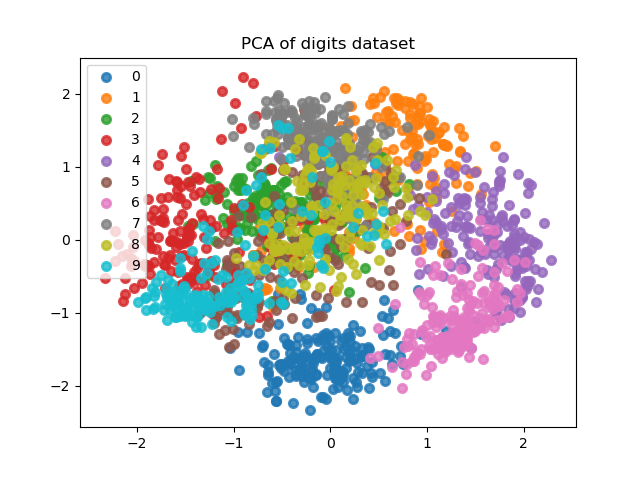
\includegraphics[scale=0.5]{images/digits_PCA.png}
				\caption{PCA Clustering of the NIST Digits Dataset. Visually, we can see that there is some clustering, but the data has a pretty high degree of similarity even after PCA.}
		\end{figure}
		
		\end{frame}
		
		\begin{frame}
			\frametitle{K Nearest Neighbors Classifier}
			
			\begin{itemize}
				\item Pre-processing:
				\begin{itemize}
					\item We split the data into a 30\% train and 70\% test sets and keep the data balanced.
					\item We also shuffle the data.
					\item We scale the data such that it is within $(0,1)$ using a min-max scaler.
				\end{itemize}
				\item The function class we consider is trivial since it is dependent only on the training data given.
				\item We can view this as a weighting function that weights the $k$-nearest points to the input with $\frac{1}{k}$ and all other points $0$.
				\item Classification Accuracy: 76 percent
				\item Training Accuracy: 83 percent
			\end{itemize}
		\end{frame}
		
		\begin{frame}
			\frametitle{Confusion Matrix for Digits Data}
			
			\begin{figure}
				\centering
				\includegraphics[scale=0.5]{images/confusion_matrix_digits.png}
				\caption{Confusion Matrix of Digit Data. We see many interesting artifacts: 0's, 4's, and 6's are classified nicely, 1's have some confusion with 7's (vice versa), 2's with 5's, 3's with 9's, 5's with 8's, 8's with 2's and 5's, and 9's with 1's and 3's.}
		\end{figure}
		\end{frame}
		
		\begin{frame}
		\frametitle{Persistence Images of Digits: 0's}
		
		\begin{figure}
				\centering
				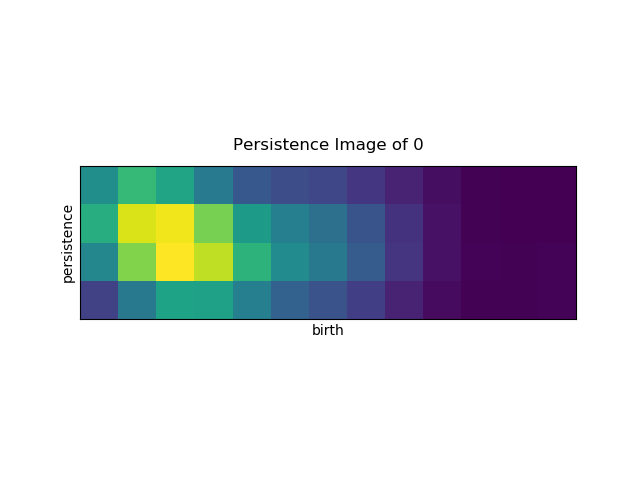
\includegraphics[scale=0.5]{images/PI_H0_0.png}
				\caption{Persistence Image for 0.}
		\end{figure}
		\end{frame}

		\begin{frame}
		\frametitle{Persistence Images of Digits: 0's}
		
		\begin{figure}
				\centering
				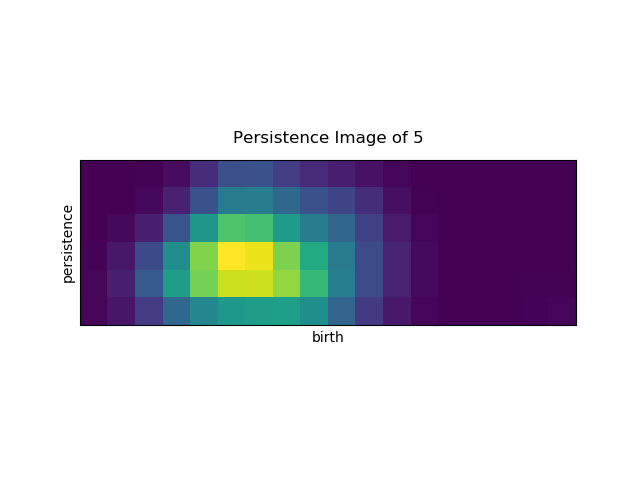
\includegraphics[scale=0.5]{images/PI_H0_5.png}
				\caption{Persistence Image for 5.}
		\end{figure}
		\end{frame}
		
		
				\begin{frame}
		\frametitle{Persistence Images of Digits: 8's}
		
		\begin{figure}
				\centering
				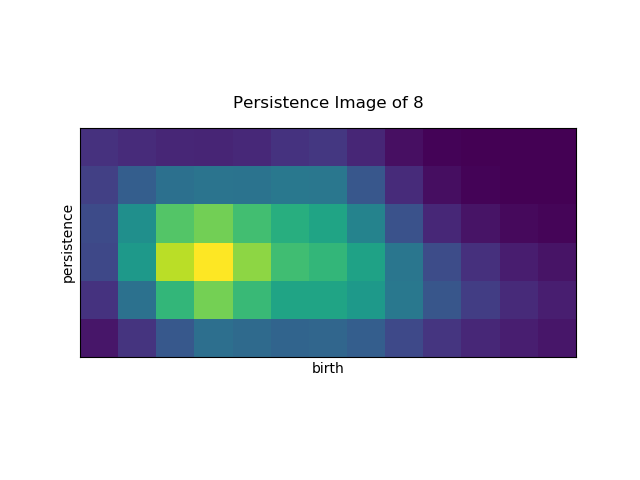
\includegraphics[scale=0.4]{images/PI_H0_8.png}
				\caption{Persistence Image for 8.}
		\end{figure}
		\end{frame}
		
				\begin{frame}
		\frametitle{Persistence Diagram of Digits: 0's, 5's, \& 8's}
		
		\begin{figure}
				\centering
				\includegraphics[scale=0.35]{images/pd058.png}
				\caption{Persistence Image for 0, 5, 8. Notice the birth/death are similar for 5 and 8 versus 0.}
		\end{figure}
		\end{frame}
		
		
		
		
		\begin{frame}
		\frametitle{Pairwise Bottleneck Distances}
		
		\begin{itemize}
			\item The bottleneck distances:
				\begin{itemize}
					\item With themselves: 0 (control)
					\item 0, 5: 2.56941795
					\item 0, 8: 2.21272278
					\item 5, 8: 2.11571217 
				\end{itemize}
		\end{itemize}
		
		A downside to the Bottleneck Distance as a measure is that quantitatively it can be hard to distinguish for simple data what a good distance is.
		\end{frame}